\section{Gibbs sampling}
\no {\bf Requirement:} $P\s(\theta)$ is difficult to sample, but after partitioning $\theta$ into two (or more) sets of parameters, $\theta_1, \theta_2, \ldots$, their conditionals, i.e. $P(\theta_1\;|\;\theta_2, \ldots)$ and $P(\theta_2\;|\;\theta_1, \ldots)$, are easy to sample.

\subsection{Gibbs sampling algorithm}
\begin{enumerate}
	\item Derive the conditional distributions $P(\theta_1\;|\;\theta_2)$, $P(\theta_2\;|\;\theta_1)$
	\item Initialize $\theta_1^{(0)}$
	\item Draw $\theta_2^{(s+1)}$ from $P(\theta_2\;|\;\theta_1^{(s)})$
	\item Draw $\theta_1^{(s+1)}$ from $P(\theta_1\;|\;\theta_2^{(s+1)})$
	\item Add $\theta^{(s+1)} = (\theta_1^{(s+1)}, \theta_2^{(s+1)})$ to the collection of samples $\{\theta^{(s)}\}$. Return to step 3.
\end{enumerate}

\subsection{Example: Triangle distribution in 2D}
\begin{itemize}
	\item Unnormalized distribution $P\s(\theta_1, \theta_2) = \text{max} (0,\;1 - |\theta_1| - |\theta_2|)$
	\item 2-dimensional Gibbs sampler: The conditionals are
		\ba
		P(\theta_1\;|\;\theta_2) &=& \text{Triangle}(\theta_1\;|\;\text{loc} = 0, \text{scale} = 1-|\theta_2|) 
		\\
		P(\theta_2\;|\;\theta_1) &=& \text{Triangle}(\theta_2\;|\;\text{loc} = 0, \text{scale} = 1-|\theta_1|),
		\ea
		where $\text{Triangle}(x\;|\;\text{loc}, \text{scale}) = \frac{1}{2}\text{max(0,\;\text{scale} - |x - \text{loc}|)}$ is the symmetric 1-d triangle distribution.
\end{itemize}
\begin{lstlisting}[language=python]
from scipy.stats import triang
def triangle(loc=0, scale=1):
    return triang(c=0.5, loc=-scale + loc, scale=2*scale)

iters = 10_000
theta1_samples = []
theta2_samples = []
theta_1 = 0
for it in range(iters):
    theta_2 = triangle(scale=1-abs(theta_1)).rvs()
    theta_1 = triangle(scale=1-abs(theta_2)).rvs()
    theta1_samples.append(theta_1)
    theta2_samples.append(theta_2)
\end{lstlisting}

\begin{figure}[h!]
\centering
	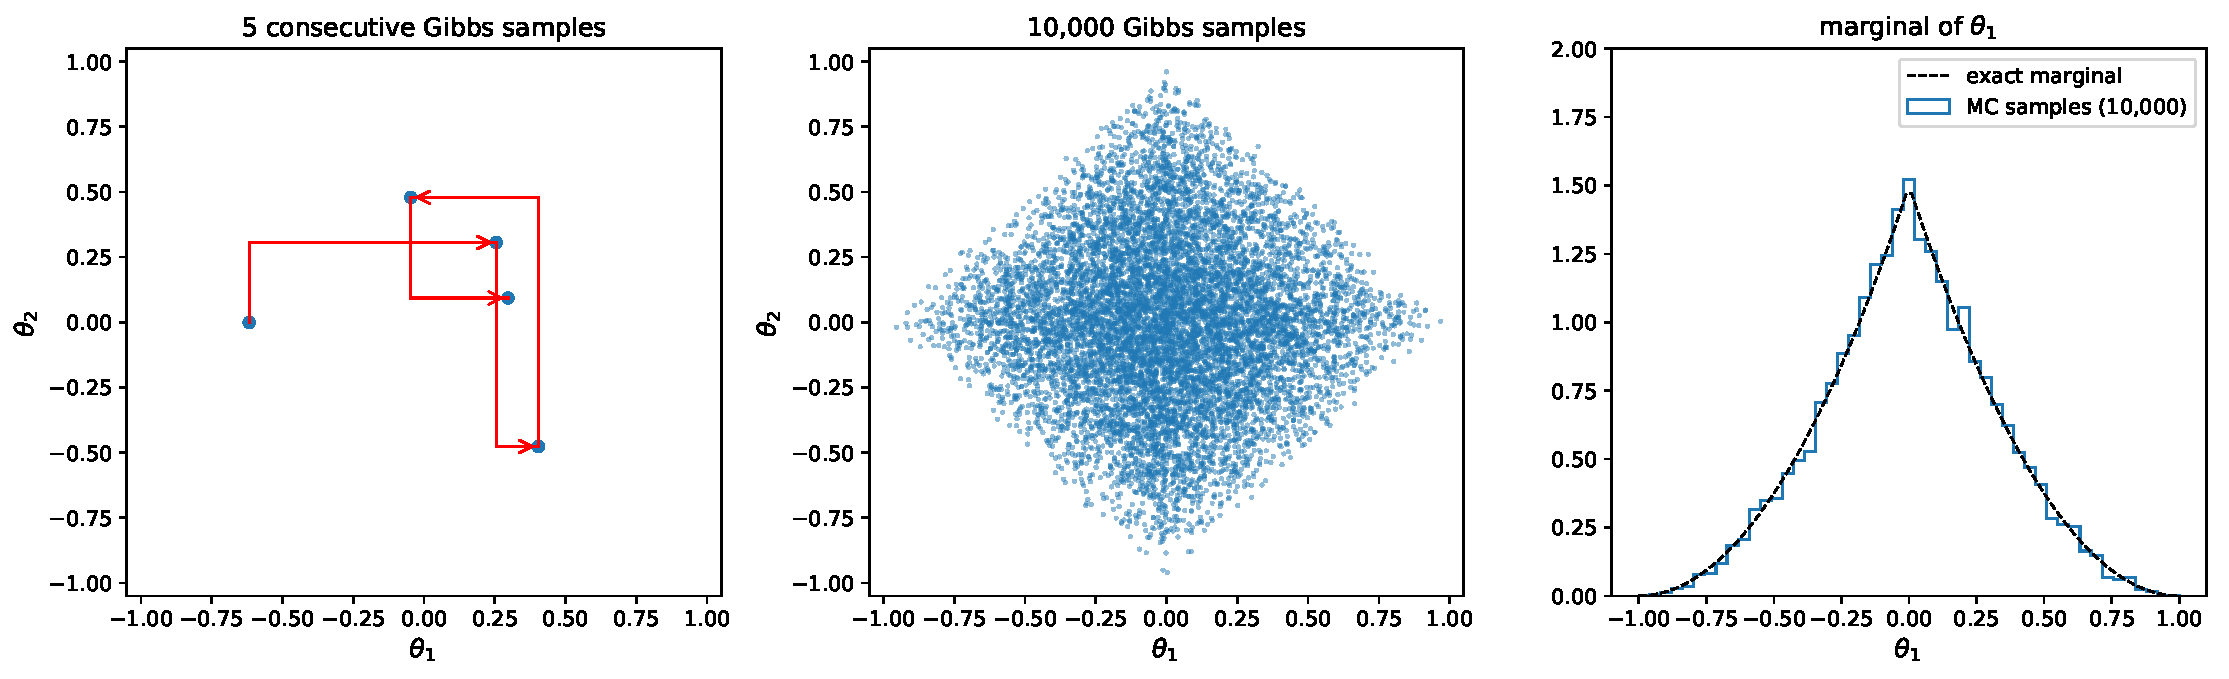
\includegraphics[width=0.95\textwidth]{./figs/08-2d-triangle.pdf}
\end{figure}

\subsection{Example: Binomial clustering}
\begin{itemize}
	\item Data: $D = \{k_i\}_{i=1}^N$, where $k_i$(successes)$ \in \{0, 1, 2, \ldots n\}$, out of $n$ trials.
	\item Parameters:
		\begin{itemize}
			\item Cluster weights: $w = \{w_c\}_{c=1}^C$, where $w_c \in [0,1]$ such that $\sum_c w_c = 1$, with flat prior, i.e. $P(w) = \text{const.}$
			\item Probability of success in each cluster: $p = \{p_c\}_{c=1}^C$, where $p_c \in [0,1]$, with a weak prior $P(p_c) = \text{Beta}(p_c\;|\;\alpha_c^{(0)}, \beta_c^{(0)})$, where $\alpha_c^{(0)}, \beta_c^{(0)}$ are small positive numbers.
			\item Hidden labels: $L = \{l_i\}_{i=1}^N$, where $l_i \in \{1,2,\ldots C\}$.
		\end{itemize}
	\item Model:
		\begin{itemize}
			\item Level 1: $P(l_i = c\;|\;w) = w_c$
			\item Level 2: $P(k_i\;|\; l_i = c,\; p) = \text{Binomial}(k_i\;|\;n, p_c)$
		\end{itemize}
		\begin{figure}[h!]
		\centering
			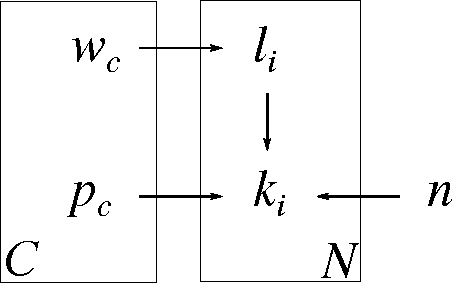
\includegraphics[height=20mm]{./figs/08-clustering.pdf}
		\end{figure}
	\item Unnormalized posterior:
	\be
		P\s(L, w, p\;|\;D) 
		\propto \left[\prod_{i=1}^N P(k_i\;|\;p_{l_i})\; P(l_i\;|\;w)\right] P(w)P(p)
		\quad\propto\quad
		\prod_{i=1}^N \text{Binomial}(k_i\;|\;n, p_{l_i}) \; w_{l_i}
	\ee
	\item Partitioning:
	\be
		\theta = (w, p, L)\qquad \rightarrow \qquad \theta_1 = (w, p),\quad \theta_2 = L
	\ee
	\item $P(\theta_1\;|\;\theta_2, \,D)$ conditionals:
	\ba
		P(w, p\;|\;L,D) &=& P(w\;|\;L) \;P(p\;|\;L, D)
		\\
		\text{where}&&
		\\
		P(w\;|\;L) &\propto& P(L\;|\;w)P(w) \propto \prod_{i=1}^N w_{l_i} = \prod_{c=1}^C (w_c)^{N_c}
		\\
		&=& \text{Dirichlet}\Big(w\;\Big|\;\alpha_c = 1 + N_c\Big)
		\\
		P(p\;|\;L, D) &\propto& P(D\;|\;L, \mu, \sigma) P(p) \propto \left[\prod_{i=1}^N \text{Binomial}(k_i\;|\;n, p_{l_i})\right]\times\left[\prod_{c=1}^C\text{Beta}(p_c\;|\;\alpha_c^{(0)}, \beta_c^{(0)})\right]
		\\
		&=& \prod_{c=1}^C \text{Beta}(p_c\;|\;\alpha = \alpha_c^{(0)} + K_c, \;\beta = \beta_c^{(0)} + nN_c - K_c),
	\ea
	where $N_c = \sum_i\delta_{l_i, c}$, \; $K_c = \sum_i \delta_{l_i, c} k_i$, where $\delta_{l_i, c} = 1$ if $l_i = c$ and 0 otherwise.

	\item $P(\theta_2\;|\;\theta_1, \,D)$ conditionals:
	\ba
		P(L\;|\;w, p, D) &\propto& P(D\;|\;L, p) \;P(L\;|\;w) = \prod_{i=1}^N \text{Binomial}(k_i\;|\;p_{l_i}) \; w_{l_i} 
		\\
		&=& \prod_{i=1}^N\text{Categorical}\left(l_i\;\Big|\; f_c = \frac{w_c\text{Binomial}(k_i\;|\;n, p_c)}{\sum_{c'}w_{c'}\text{Binomial}(k_i\;|\;n, p_{c'})}\right)
	\ea
	\item Gibbs sampling:
\end{itemize}

\begin{lstlisting}[language=python]
import numpy as np
from numpy.random import choice
from scipy.stats import binom, beta, dirichlet

def sample_labels(k_data, n, w, p):
    labels = []
    for ki in k_data:
        f = w * binom.pmf(ki, n, p)
        f /= np.sum(f)
        labels.append(choice(clusters, p=f))
    return np.array(labels)

def sample_w(labels, clusters):
    alpha = []
    for c in clusters:
        alpha.append(1 + np.sum(labels == c))
    return dirichlet.rvs(alpha)[0]

def sample_p(labels, k_data, n, clusters, alpha0, beta0):
    N = len(k_data)
    p = []
    for c in clusters:
        Kc = np.sum(k_data[labels == c])
        Nc = np.sum(labels == c)
        a = alpha0[c] + Kc
        b = beta0[c] + n*Nc - Kc
        p.append(beta.rvs(a, b))
    return np.array(p)

clusters = list(range(3))
alpha0 = [0, 0.5, 1]
beta0 = [1, 0.5, 1]

w = np.array([1./3] * 3 )
p = np.array([0.01, 0.5, 0.6])

labels_samples = []
w_samples = []
p_samples = []
iters = 100
for it in range(iters):
    labels = sample_labels(k_data, n, w, p)
    w = sample_w(labels, clusters)
    p = sample_p(labels, k_data, n, clusters, alpha0, beta0)
    labels_samples.append(labels)
    w_samples.append(w)
    p_samples.append(p)
\end{lstlisting}

\begin{figure}[h]
\centering
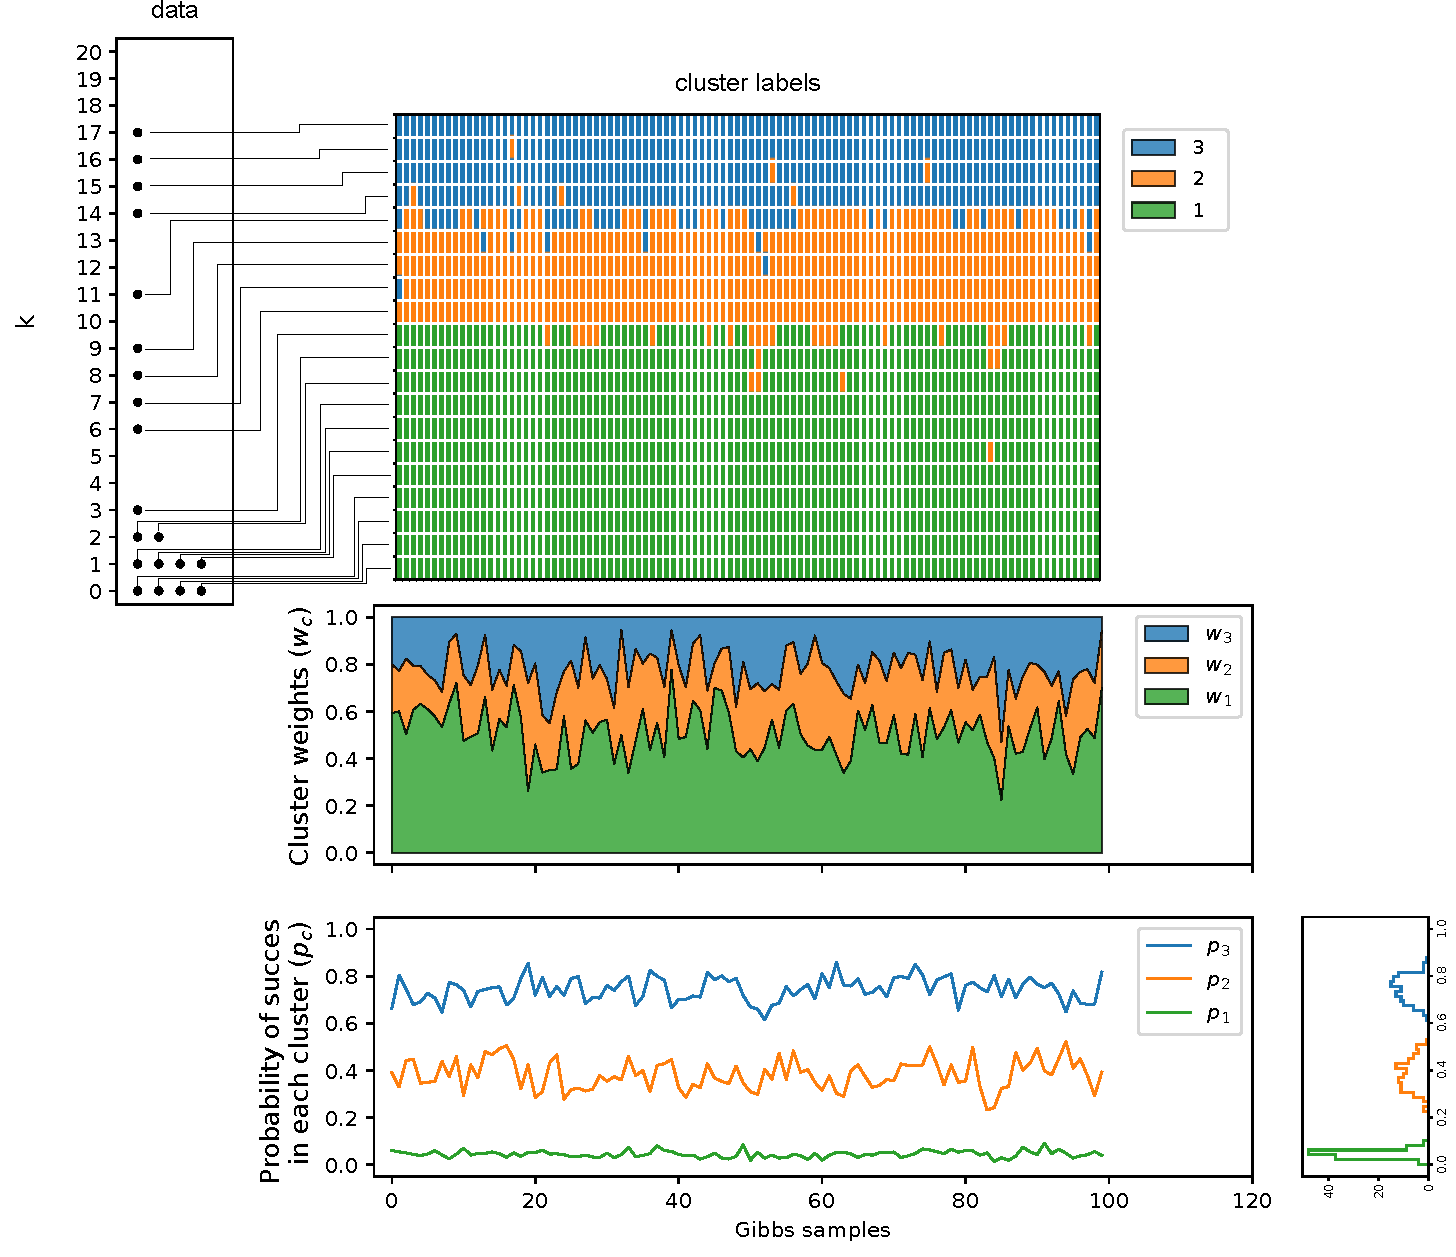
\includegraphics[width=\textwidth]{./figs/08-gibbs-binomial-samples.pdf}
\end{figure}

\begin{figure}[h]
\centering
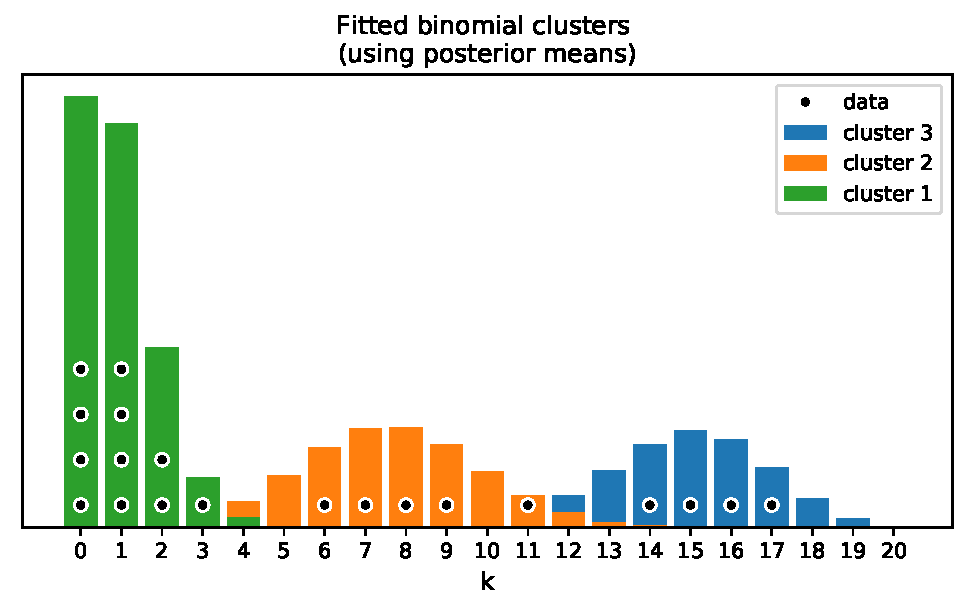
\includegraphics[width=0.7\textwidth]{./figs/08-binomial-clustering-posterior.pdf}
\end{figure}




